\Lecturer{Hui Jin}
\Contributor{}
\LectureNumber{14}
\LectureDate{DATE}
\LectureTitle{Shor's Factoring Algorithm}

\lstset{style=mystyle}


	\MakeScribeTop

%#############################################################
%#############################################################
%#############################################################
%#############################################################

\section{Introduction}
Shor's factoring algorithm is one of the most important quantum algorithms ever discovered and is widely regarded as a landmark result in quantum computing. In principle, a sufficiently large fault-tolerant quantum computer running Shor's algorithm could break RSA, one of the most widely used public-key cryptosystems in modern Internet security. The possibility of large-scale quantum computers has motivated significant research into post-quantum cryptography, which aims to develop cryptographic systems resistant to quantum attacks. 

The RSA algorithm relies on a simple yet profound idea: prime factorization is a practically hard problem. Although an elementary school student understands the basic idea of factorization, the actual computation to factor a large number involves an insurmountable computation, at least for all known algorithms on a classical computer. 

Here is the problem statement: given a number \(N\), and the knowledge that \(N\) is a product of two prime numbers \(p, q\), how do we find these two primes? 

The best known classical factoring algorithms require super-polynomial time in the number of bits of N. 

Shor's factoring algorithm running on a quantum computer has complexity: 
\begin{align*}
    \mbox{Quantum Complexity}_N = O((\log N)^3),
\end{align*}
which is polynomial complexity. Therefore quantum algorithm achieves an exponential speedup over classical algorithms. 

\section{Shor's factoring algorithm overview}
At its core, Shor's prime factorization algorithm is a sub-quantum routine that finds the order of an integer in the ring \(Z_N\). 

\begin{lemma}
Given \(N\), which is odd and not a power of a prime, and an integer \(a < N\), where  \(GCD(a, N) = 1\). The order \(r\) of \(a\) is defined as the minimum  \(r\) such that
\begin{align*}
    a^{r} \equiv 1 \pmod{N}
\end{align*}
\end{lemma}

Knowing the order, the other parts of Shor's factoring algorithm rely on classical computers, with polynomial complex. Here is the overview of Shor's factoring algorithm.


So the key step is the order finding algorithm, which can be solved in polynomial time on a quantum computer. The quantum algorithm relies on the quantum phase estimation. By before we can describe the phase estimation quantum algorithm, we first need to describe quantum Fourier transform.



\section{Quantum Fourier Transform}
A classical discrete Fourier Transform (DFT) linearly maps a vector of length \(N\) \(x = (x_0, x_1, \cdots x_{N-1})\) to another vector length \(N\) \(y=(y_0, y_1, \cdots, y_{N-1})\) by the following transformation: 
\begin{align*}
    y_j = \sum_{k=0}^{N-1} \omega_{N}^{kj} x_k,
\end{align*}
for \(j=0, 1, \cdots, N-1\), where \(\omega_{N} = e^{2\pi i/N}. \)

Similarly, the quantum Fourier Transform has the same form, where it maps the (superposition) state of \(n=\log_2 N\) qubits
\begin{align}
    \ket{x} = \sum_{i=0}^{N-1} x_i \ket{i}
\end{align}

to another state of \(n\) qubits:
\begin{align}
    \ket{y} = \sum_{i=0}^{N-1} y_i \ket{i}
\end{align}
by the following transformation: 
\begin{align*}
    y_j = \frac{1}{\sqrt{N}} \sum_{k=0}^{N-1} \omega_{N}^{kj} x_k,
\end{align*}
for \(j=1, \cdots, N\), where \(\omega = e^{2\pi i/N}. \) Note that to make the transformation a unitary operation, we introduced a normalization factor \(\frac{1}{\sqrt{N}}\) compared to conventional discrete Fourier transform. 

As quantum circuit has linear property, we can focus on the input of quantum Fourier Transform being basis state \(\ket{x}\), where \(x\) is an integer between \(0\) and \(N-1\), then each \(y_j\) equals to \(\omega_N^{xj}\). Like \(\ket{x}\) where we abuse the notion a bit by assuming it is the base state now, let us use \(\ket{y}\) to denote \(j\). Then the quantum Fourier transform can be equivalently described as a linear mapping between base states \(\ket{x}\) and \(\ket{y}\):
\begin{align}
    \mbox{QFT: } \ket{x} \rightarrow \frac{1}{\sqrt{N}} \sum_{y=0}^{N-1} \omega_{N}^{xy} \; \ket{y}.
    \label{eq:baseState}
\end{align}
Similar to Hadamard transform, a QFT maps a basis state to a superposition of base states with a distinct structure. In fact it is informative to compare the Hadamard transform mapping:
\begin{align*}
    H_N: \ket{x} \rightarrow \frac{1}{\sqrt{N}} \sum_{y=0}^{N-1} (-1)^{x \cdot y} \; \ket{y},
\end{align*}
where \(x\cdot y\) is an inner product of the \(x, y\) binary representation vector.

As we know the mapping of the basis state \(\ket{x}\) picks up the \(x\) column of the unitary matrix, Eq.~\ref{eq:baseState} reveals that the unitary matrix (or quantum gates) for the QFT is: 
\begin{align}
\frac{1}{\sqrt{N}}
\begin{pmatrix}
1 & 1 & 1 & \cdots & 1 \\
1 & \omega_N & \omega_N^2 & \cdots & \omega_N^{N-1} \\
1 & \omega_N^2 & \omega_N^4 & \cdots & \omega_N^{2(N-1)} \\
\vdots & \vdots & \vdots & \ddots & \vdots \\
1 & \omega_N^{N-1} & \omega_N^{2(N-1)} & \cdots & \omega_N^{(N-1)^2}
\end{pmatrix}.    
\label{eq:QFT}
\end{align}

\begin{example} \(1\) qubit ((N=2))
Since \(\omega_2=e^{\pi i}=-1\),
\[\mbox{QFT}_2 = 
\frac{1}{\sqrt{2}}
\begin{pmatrix}
1 & 1\\
1 & -1
\end{pmatrix}.
\]
This is exactly the Hadamard gate.
\end{example}


\begin{example}
2 qubits ((N=4)).

Here \(\omega_4=i\), so
\[ \mbox{QFT}_4 = 
\frac{1}{2}
\begin{pmatrix}
1 & 1 & 1 & 1\\
1 & i & -1 & -i\\
1 & -1 & 1 & -1\\
1 & -i & -1 & i
\end{pmatrix}.
\]
\end{example}


\subsection{Implementation of Quantum Fourier Transform}
The quantum circuit corresponding to the unitary matrix Eq.~\ref{eq:QFT} is known as the QFT quantum circuit. The structure can be defined in a recursive manner. The core technique involved is reminiscent of the Fast Fourier Transform. 

Let's look at the mapping Eq~\ref{eq:baseState}. We claim that it can be decomposed as a tensor product of \(n\) qubits, just like Hadamard transform. Unlike Hadamard transform, where each qubit is a \(\ket{+}\) or \(\ket{-}\) in the Tensor product, here each qubit is in the form of \(\ket{0} + e^{2\pi i \; 0.x_{k-1}\cdots x_0} \ket{1}\), where \(0.x_{k-1}\cdots x_0 = 2^{-1}x_{k-1} + 2^{-2}x_{k-2}+ \cdots + 2^{-k}x_0.\)

In fact, we rewrite Eq~\ref{eq:baseState} as: 
\begin{align*}
    \mbox{QFT } \ket{x} &= \frac{1}{\sqrt{2^n}} \sum_{y=0}^{2^n-1} \omega_{2^n}^{xy} \; \ket{y} \\
    &= \frac{1}{\sqrt{2^n}} \sum_{y=0}^{2^n-1} e^{2\pi i \frac{xy}{2^n}} \; \ket{y} \\
    &= \frac{1}{\sqrt{2^n}} \sum_{y_0=0}^{1}\sum_{y_1=0}^{1}\cdots\sum_{y_{n-1}=0}^{1}  e^{2\pi i \frac{x(2^{n-1} y_{n-1} +2^{n-2} y_{n-2} + \cdots + y_0)}{2^n}} \; \ket{y_{n-1}y_{n-2}\cdots y_0} \\
    &= \frac{1}{\sqrt{2^n}} 
    (\ket{0} + e^{2\pi i x \frac{1}{2}}\ket{1})\otimes
    (\ket{0} + e^{2\pi i x \frac{1}{4}}\ket{1}) \otimes
    \cdots 
    (\ket{0} + e^{2\pi i x \frac{1}{2^{n-1}}}\ket{1}) \\
    &= \frac{1}{\sqrt{2^n}} 
    (\ket{0} + e^{2\pi i \; 0.x_0}\ket{1})\otimes
    (\ket{0} + e^{2\pi i \;0.x_1x_0}\ket{1}) \otimes
    \cdots 
    (\ket{0} + e^{2\pi i \;0.x_{n-1}x_{n-2}\cdots x_0}\ket{1}). 
\end{align*}
Here \((\ket{0} + e^{2\pi i \; 0.x_0}\ket{1})\) corresponds to the \(n\)-th qubit \(\ket{y_{n-1}}\), \((\ket{0} + e^{2\pi i \; 0.x_1x_0}\ket{1})\) corresponds to the \((n-1)\)-th qubit \(\ket{y_{n-2}}\), and so on. So the mapping involves a reverse ordering. 

The implementation now uses a controlled phase shift quantum gate (CP). 


A normal phase shift quantum gate has the following property: 
\[\mbox{Phase Shift}: \ket{0} + \ket{1} \rightarrow \ket{0}+ e^{i \theta} \ket{1}.\]


In contrast, a controlled-phase shift quantum gate introduces a control qubit, with the following unitary matrix: 
\[ \mbox{CP} = 
\begin{pmatrix}
1 & 0 & 0 & 0\\
0 & 1 & 0 & 0\\
0 & 0 & 1 & 0\\
0 & 0 & 0 & e^{i\theta}
\end{pmatrix}.
\]
Here is the mapping of the basis states for a controlled-phase shift of \(\theta\): 
\begin{align*}
  \mbox{CP}\ket{00} &= \ket{00} \\
  \mbox{CP}\ket{01} &= \ket{01} \\
  \mbox{CP}\ket{10} &= \ket{10} \\
  \mbox{CP}\ket{11} &= e^{i \theta} \ket{11} 
\end{align*}

Let's see how we implement the qubits in 
\[
\frac{1}{\sqrt{2^n}} 
    (\ket{0} + e^{2\pi i \; 0.x_0}\ket{1})\otimes
    (\ket{0} + e^{2\pi i \;0.x_1x_0}\ket{1}) \otimes
    \cdots 
    (\ket{0} + e^{2\pi i \;0.x_{n-1}x_{n-2}\cdots x_0}\ket{1}). 
\]
Assume we order the qubits as \(\ket{x_{n-1}}, \ket{x_{n-2}} \cdots \ket{x_0}\), where \(\ket{x_{n-1}}\) is on the top branch and \(\ket{x_0}\) is at bottom, then we can obtain \(\ket{y_0} = \ket{0} + e^{2\pi i \;0.x_{n-1}x_{n-2}\cdots x_0}\ket{1}\) on the top branch by implementing a Hadamard transform on \(\ket{x_{n-1}}\), followed by a \(\ket{x_{n-2}}\) controlled phase shift of \(e^{2\pi i/4}\), followed by a \(\ket{x_{n-3}}\) controlled phase shift of \(e^{2\pi i/8}\), and so on, the last one \(\ket{x_{0}}\) controlled phase shift of \(e^{2\pi i/2^{n}}\). A similar circuit generates the \(k-th\) qubit \(\ket{y_{k-1}}\). In order to have the qubits ordered from \(\ket{y_{n-1}}, \ket{y_{n-2}}, \cdots, \ket{y_0}\), we do pair-wise swapping: swap the top and bottom qubits, the second top and second bottom, and so on. 

\begin{figure}[h]
    \centering
    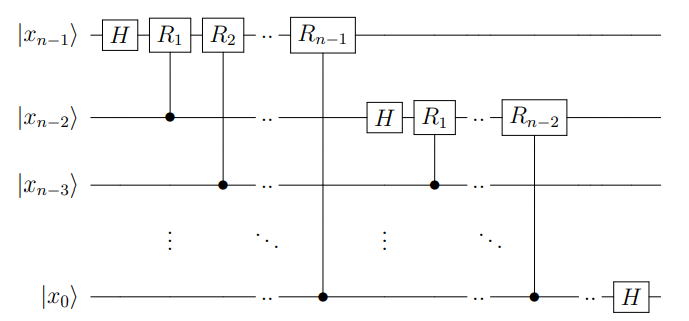
\includegraphics[width=0.85\textwidth]{Figs/QFT.png}
    \caption{Quantum Fourier Transform. Here \(R_k\) represents controlled-phase shift gate with phase \(2\pi /2^{k+1}\). Qubits here are indexed from \(0\) to \(n-1\).}
    \label{fig:PEA}
\end{figure}


\section{Phase Estimation Problem}
The quantum phase estimation problem, 
\begin{lemma}
Given a quantum circuit \(U\) and an eigenvector \(\ket{\psi}\) that satisfies:
\begin{align*}
    U \ket{\psi} = e^{2\pi i \theta} \ket{\psi}  
\end{align*}
we have an efficient way to approximate \(\theta\). The approximation \(\theta \approx \frac{y}{2^m}\) has error less than \(\frac{1}{2^m}\), where \(m\) is the number of qubits used for this approximation.      
\end{lemma}

Here we assume \(\ket{\psi}\) is provided and promised to be an eigenvector. It means that we have \(\ket{\psi}\) as the input to a quantum circuit. 

A basic diagram for the quantum phase estimation is depicted in Figure~\ref{fig:PEA}, for \(m=3\). One of the critical module used is the \(QFT^{-1}\), the inverse quantum Fourier Transform. We shall first describe it in the next section before we come back to the details of quantum phase estimation.
\begin{figure}[h]
    \centering
    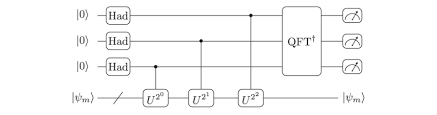
\includegraphics[width=0.85\textwidth]{Figs/PEA.png}
    \caption{Quantum Phase Estimation Circuit for \(m=3\). Estimation precision can be increased by increasing \(m\), along with complexity.}
    \label{fig:PEA}
\end{figure}

The key principle here is the phase kick-back mechanism. 
For example, a single control qubit running a controlled-\(U^{2^k}\) acts globally as:
\begin{align*}
CU^{2^k} \ket{0}\ket{\psi} &\rightarrow \ket{0}{\psi} \\
CU^{2^k} \ket{1}\ket{\psi} &\rightarrow e^{2\pi i (2^k \theta)} \ket{1}\ket{\psi} \\ CU^{2^k} (\ket{0}+\ket{1})\ket{\psi} &\rightarrow (\ket{0}+e^{2\pi i (2^k \theta)}\ket{1})\ket{\psi} 
\end{align*}
We see that the controlled-\(U^{2^k}\) gate injects a phase shift into the controlled qubit. 

Therefore, we can write down the system state after each controlled-\(U^{2^k}\) operation. Before the first controlled operation, the state is 
\begin{align*}
    \ket{+}\ket{+}\ket{+}\ket{\psi_m}
\end{align*}
After the first controlled operation \(U^{2^0}\) by the third qubit, the quantum state is:
\begin{align*}
    \ket{+}\ket{+}(\ket{0} + e^{2\pi i\theta}\ket{1})\ket{\psi_m}
\end{align*}
After the second controlled operation \(U^{2^1}\) by the second qubit, the quantum state is:
\begin{align*}
    \ket{+}(\ket{0} + e^{2\pi i 2\theta}\ket{1})(\ket{0} + e^{2\pi i\theta}\ket{1})\ket{\psi_m}
\end{align*}

Finally after the third controlled operation \(U^{2^2}\) by the first qubit, the quantum state is:
\begin{align*}
    (\ket{0} + e^{2\pi i 4\theta}\ket{1})(\ket{0} + e^{2\pi i 2\theta}\ket{1})(\ket{0} + e^{2\pi i\theta}\ket{1})\ket{\psi_m}
\end{align*}
Looking at the first qubits closely, we realize that this is exactly (up to a constant scaling \(\frac{1}{\sqrt{2^n}}\)), the quantum Fourier transform of base state \(\ket{y}\), where \(\theta\) is approximated by an m-bit integer \(y\), in other words \(\theta \approx y/2^m\). Therefore, the inverse Fourier transform recovers the basis state \(\ket{y}\)!

The above algorithm is exact and deterministic if \(\theta = \frac{y}{2^m}\). When \(\frac{y-1}{2^m} < \theta < \frac{y}{2^m}\), then the measure of the \(m\)-th qubit is probabilistic. By increasing \(m\), we improve the approximation accuracy.

\section{Quantum Order Detection}
The quantum phase estimation algorithm facilitates an efficient solution of a classically difficult number theory problem - finding the order of a number \(a\) in \(Z_N\). For integer \(1\leq a < N\), the order of \(a\) of modulus \(N\) is defined as the minimum number \(r\) such that 
\begin{align*}
    a^r \equiv 1 \pmod {N}
\end{align*}

\subsection{Unitary operation and its Eigenvectors}
We define the mapping \(U_a\) as:
\begin{align*}
    U_a \ket{k} = \ket{ak}  \pmod{N}, 
\end{align*}
for \(k=0, 1, \cdots, N-1.\)
Since \(U_a\) corresponds to a permutation matrix, it is unitary and must corresponds to a quantum circuit. 

Let's try to find the eigenvectors and their corresponding eigenvalues of this unitary matrix. 

Consider 
\begin{align*}
    \ket{\psi_j} = \frac{1}{\sqrt{r}} \sum_{k=0}^{r-1} \omega_r^{-jk}\ket{a^k},
\end{align*}
where \(\omega_r = e^{2\pi i \frac{1}{r}}.\)

If we apply \(U_a\) on qubits \(\ket{\psi_j}\), we have 
\begin{align*}
    U_a \ket{\psi_j} &= \frac{1}{\sqrt{r}} \sum_{k=0}^{r-1} \omega_r^{-jk}\ket{a^{k+1}}\\
    &= \omega_r^{j} \frac{1}{\sqrt{r}} \sum_{k=0}^{r-1} \omega_r^{-jk}\ket{a^k} \\
    &= \omega_r^{j} \ket{\psi_j}.
\end{align*}
That means \(\ket{\psi_j}\) is an eigenvector with eigenvalue \(\omega_r^{j} = e^{2\pi i \frac{j}{r}}\).

If the eigenvector is prepared properly, we can use the phase estimation algorithm to extract the phase \(\frac{j}{r}\) by approximating it to a number \(\frac{y}{2^m}\). If \(m\) is sufficiently large, \(\frac{j}{r}\) can be extracted exactly from \(\frac{y}{2^m}\).


\subsection{Continued Fraction Extraction}

The quantum measurement step yields an estimate $\phi \approx \frac{j}{r}$ formatted as a dyadic fraction $\frac{y}{2^m}$. To extract the true period $r$ from this measured value, we use the classical **Continued Fractions Algorithm**.

The continued fraction expansion expresses the measured ratio $\frac{y}{2^m}$ as a nested fraction:
\begin{align*}
    \frac{y}{2^m} = a_0 + \cfrac{1}{a_1 + \cfrac{1}{a_2 + \cfrac{1}{a_3 + \dots}}}
\end{align*}
Truncating this expansion at successive depths produces a sequence of rational approximations $\frac{p_k}{q_k}$ known as *convergents*. By choosing a register size $m \geq 2\log_2 N + 1$, bounded error properties guarantee that the true fraction $\frac{j}{r}$ appears explicitly as one of these unique convergents $\frac{p_k}{q_k}$.

The classical post-processing steps are executed as follows:
\begin{enumerate}
    \item Compute the sequence of convergents $\frac{p_k}{q_k}$ for the measured fraction $\frac{y}{2^m}$.
    \item For each convergent with a denominator $q_k < N$, test whether $q_k$ serves as the valid period by checking if $a^{q_k} \equiv 1 \pmod{N}$.
    \item If the condition holds, set $r = q_k$. If $j$ and $r$ share a common factor, the convergent will reduce to a simplified form $\frac{p_k}{q_k} = \frac{j/d}{r/d}$. In this scenario, the test fails, and the algorithm is restarted. Over multiple runs, the probability of sampling a coprime value for $j$ is sufficiently high to guarantee finding the correct period $r$ in $O(1)$ repetitions.
\end{enumerate}

\section{Period finding: A problem at the heart of quantum computing}
While trends may have moved on, the idea of extracting group structure from the Fourier spectrum is still at the very core of what quantum computers could be useful for. Scott Aaronson, for example, in his 2022 commentary “How Much Structure Is Needed for Huge Quantum Speedup?” presents the following hierarchy:

 \begin{figure}[h]
    \centering
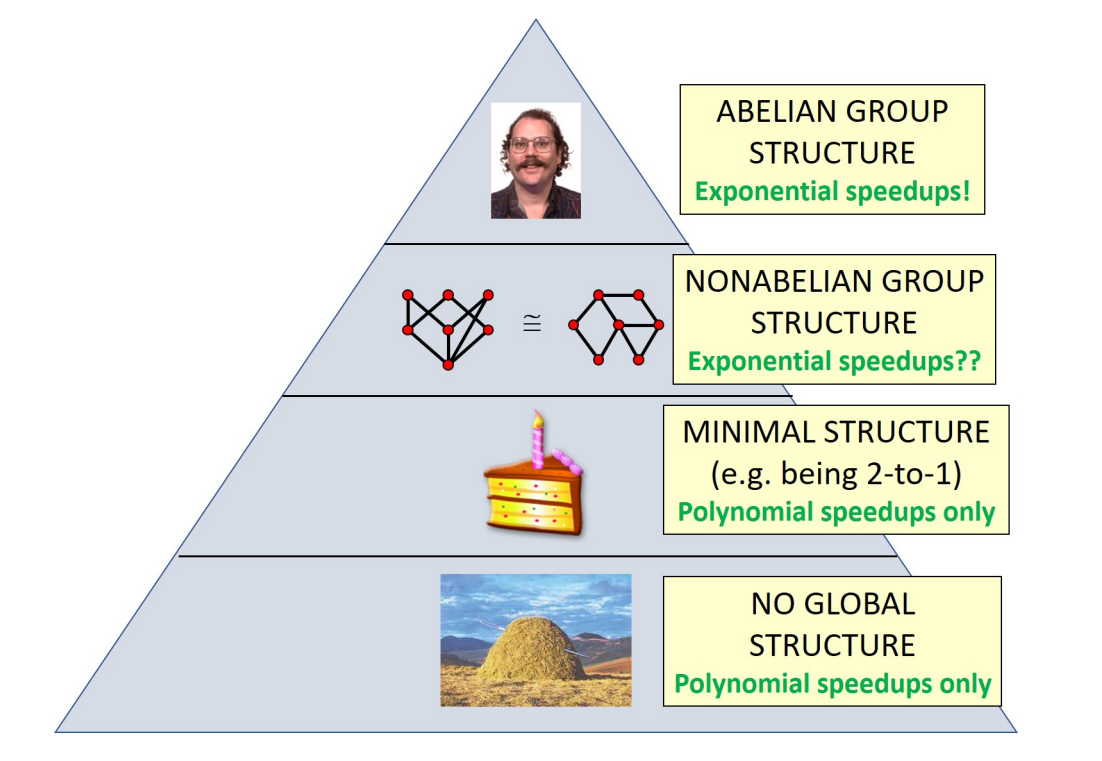
\includegraphics[width=0.6\textwidth]{Figs/aaronson_fig6.png}
    \caption{Speedup.}
    \label{fig:QFT}
\end{figure}




















    
